\mode<all>
% Incluyo los paquetes necesarios.
% para no tener problemas con acentos etc.
\usepackage[utf8]{inputenc}
% en español
\usepackage[spanish]{babel}
%matemática
\usepackage{amsmath}
% este no se si hace falta pero por las dudas
\usepackage{graphicx}
% para incluir peliculas
\usepackage{multimedia}
% para usar segunda pantalla
\usepackage{pgfpages}
\usepackage{pgf}
% para hacer dibujitos
\usepackage{tikz}
\usetikzlibrary[automata,calc,arrows,decorations.pathmorphing,backgrounds,shapes,
patterns,positioning,fit,petri,overlay-beamer-styles]
\tikzstyle{every picture}+=[remember picture]
%recuadros sencillos
%\usepackage{tcolorbox}
% enumeradores intercambiables
\usepackage{enumerate}
% para subtitulos en figuras
\usepackage{subcaption}
%listings for code input
\usepackage{listings}
%verbatim input from file!
\usepackage{verbatim}
\usepackage{fancyvrb}
% para modificar los encabezados y pies de página.
%\usepackage{fancyhdr}
%\pagestyle{fancy}
\usepackage{standalone}

\definecolor{codegreen}{rgb}{0,0.6,0}
\definecolor{codegray}{rgb}{0.5,0.5,0.5}
\definecolor{codepurple}{rgb}{0.58,0,0.82}
%\definecolor{backcolour}{rgb}{0.95,0.95,0.0.1}

\lstset{
    basicstyle=\fontsize{8}{10}\selectfont\ttfamily, 
    backgroundcolor=\color{Beige},   
    frame=lines,
    commentstyle=\color{codegreen},
    keywordstyle=\color{magenta},
    numberstyle=\tiny\color{codegray},
    stringstyle=\color{codepurple},
    breakatwhitespace=false,         
    breaklines=true,                 
    captionpos=b,                    
    keepspaces=true,                 
    numbers=left,                    
    numbersep=5pt,                  
    showspaces=false,                
    showstringspaces=false,
    showtabs=false,                  
    tabsize=4
}



\usepackage{float}
%\mode<presentation>{
% para ver las notas con la presentacion.  
%\setbeameroption{hide notes}
%para dejar las notas en la segunda patnalla
%}

% incluyo los beamercolors
%%%%%%%%%% BEAMERCOLORS
% el recuadro para el titulo
\setbeamercolor{title}{fg=white,bg=Purple}
% el recuadro para el subtitulo
\setbeamercolor{subtitle}{fg=white,bg=DarkOliveGreen}
% los títulos de las secciones tienen su colorinche:
\setbeamercolor{sectionbox}{fg=white,bg=Purple}
% cada diapositiva tendrá su color de título.
\setbeamercolor{frametitle}{fg=white,bg=ForestGreen}
% el título de las secciones tienen también su color. 
\setbeamercolor{sectiontitle}{fg=white,bg=violet}

%%%% CUSTOM BEAMERCOLORS
% estos cuadros los defino para ubicar al lector en los temas que se tratan
% son los cuadritos que aparecen arriba del título. 
\setbeamercolor{structure0}{fg=white,bg=gray}
\setbeamercolor{structure1}{fg=black,bg=DarkGray}
\setbeamercolor{structure2}{fg=black,bg=lightgray}
% defino un cuadro para usar en alguna oportunidad, creo que para titulos. 
\setbeamercolor{whitebox}{fg=black,bg=white}
% un cuadro para resaltar
\setbeamercolor{highlight1}{fg=black,bg=Gold}

% beamer colors for headers and etc.
\setbeamercolor{header1}{fg=white,bg=Blue}
\setbeamercolor{header2}{fg=black,bg=Red}
\setbeamercolor{header3}{fg=black,bg=ForestGreen}

%code block
\setbeamercolor{codeblock}{fg=Blue, bg=Beige}
\setbeamerfont{codeblock}{family=\ttfamily,size=\scriptsize}


%incluyo el tema y modificaciones
%%% BEAMER THEME
% el tema 'boxes' es igual al default pero permite definir boxes de estructura 
% a mano. 
\mode<presentation>{
  \usetheme{boxes}
  % los boxes que identifican lo que se esta leyendo
    % box de la izquierda: la materia (subtitulo)
    \addheadbox{structure2}{\quad \tiny \insertshortsubtitle}
  %  box del medio en cabecera, el titulo de la clase
    \addheadbox{structure0}{\quad \tiny  \inserttitle \quad } 
  % box en a la derecha , eltítulo de la sección. 
    \addheadbox{structure1}{\quad \tiny \insertsection}
}
% tema interno y de colores para las diapositivas normales. 
\useinnertheme{rectangles}
\usecolortheme{dove}
% la fuente de las ecuaciones
\usefonttheme[onlymath]{serif}

% entorno codeblock para meter piezas de código.
% el color se definió en BEAMERCOLORS

\newenvironment{codeblock}
{
  \begin{beamercolorbox}{codeblock}
    \usebeamerfont{codeblock}
}
{
  \end{beamercolorbox}
}



% modifico los temas
  \titlegraphic{%
\includegraphics[width=0.25\textwidth]{./PREAMBLE/logo-isabt25.png}
                
\includegraphics[width=0.25\textwidth]{./PREAMBLE/logo-isabato.png}
  		\hfill
		
\includegraphics[width=0.25\textwidth]{./PREAMBLE/ISOLOGOCNEA.png}
		\hfill
  		
\includegraphics[width=0.25\textwidth]{./PREAMBLE/unsam-horizontal.png}}

\mode<presentation>{
\setbeamertemplate{title page}[center]
{
  %
\includegraphics[width=0.25\textwidth]{./PREAMBLE/ISOLOGOCNEA.png}
  \inserttitle
  \insertsubtitle
  \insertauthor
  \insertinstitute
%  \inserttitlegraphic
}
}


% defino el template para las dapositivas con los titulos de las secciones. 
%es una recetita que saqué de algun lado. 
\setbeamertemplate{section page}{
  \begin{beamercolorbox}[ht=5ex,dp=1ex,wd=\paperwidth,center]{sectionbox}
    \begin{centering}
     \usebeamerfont{section  title} \insertsection 
    \end{centering}
  \end{beamercolorbox}
}
\AtBeginSection[]{
  \begin{frame}[plain]
    \begin{center}
    \quad \inserttitle \quad  
    \end{center}
    \sectionpage
  \end{frame}
}

% remover los simbolos de navegacion
% porque sacan espacio 
\mode<presentation>{
\setbeamertemplate{navigation symbols}{}
\setbeamertemplate{footline}[page number]
% me gustan los titulos a la derecha
\setbeamertemplate{frametitle}[default][right]%{
}
\mode<handout>{
 \setbeamertemplate{headline}{}
 \setbeamertemplate{frametitle}{}
 \setbeamertemplate{background}{
   \tikz\node [rectangle,minimum width=0.995\paperwidth,
   minimum height=0.995\paperheight,draw,anchor=south west,
   line width=2pt]  {};
 }
 \setbeamertemplate{footline}{}
}
% aparentemente el siguiente beamertemplate
%se ejecuta en modo artículo. habría que ver
%la forma de sacale probecho. 
% notar que vale solo para las framesque se incluyen 
% directamente en el artículo y no vale para 
% \includeslide.
% \setbeamertemplate{frame begin}
% \setbeamertemplate{frame end}


% no se si es el mejor lugar para definirlo, 
% pero las \includeslides deben quedar fijas al
% tamaño de la página:

%\mode<article>{
%\renewcommand\includeslide[1]{
%  \includeslide[width=\textwidth]{#1}
%}
%}

% defino el template para la diapositiva del título

%%%%%%%%%%%%%%%%%%%%%%%%%%%%%%%%
% Defino la Clase
%%%%%%%%%%%%%%%%%%%%%%%%%%%%%%%%
\subtitle[Modelización 2020]{ Modelización de Propiedades y Procesos 2021 }
\author{Ruben Weht\inst{1,2} \and Mariano Forti\inst{1,3} }
\institute{
%  \inst{1}Instituto de Tecnología Prof. Jorge Sabato
%  \and
  \inst{1}Fisica del Sólido, Edificio TANDAR, \url{weht@cnea.gov.ar},
  interno 7104
  \and
  \inst{2}División Aleaciones Especiales, Edificio 47 (microscopía),
  \url{mforti@cnea.gov.ar}, interno 7832
}

\mode<presentation>{\date{}}

\mode<article>{
  \date{
    \small
%  \textsuperscript{1} Instituto de Tecnología Prof. Jorge Sabato\\
  \textsuperscript{1}Fisica del Sólido, Edificio TANDAR, \url{weht@cnea.gov.ar},
  interno 7104 \\
  \textsuperscript{2}División Aleaciones Especiales, Edificio 47 (microscopía),
  \url{mforti@cnea.gov.ar}, interno 7832
}

%defino los encabezados y pies de págna para
% dodo el documento en función de la materia y la
% clase.
%\fancyhead[L]{\tiny Modelización de Materiales 2019}
%\fancyhead[R]{\tiny \leftmark}
}

\title{
  \mode<article>{
% 
\includegraphics[height=1cm]{./PREAMBLE/logo-isabt25.png}
    
\includegraphics[height=1cm]{./PREAMBLE/logo-isabt25.png}
\hfill

\includegraphics[height=1cm]{./PREAMBLE/ISOLOGOCNEA.png}
\hfill
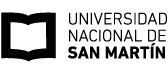
\includegraphics[height=1cm]{./PREAMBLE/logo-unsam.png}
\\} Solución de Ecuaciones Diferenciales Ordinarias }
\subject{ Métodos de Euler y de Runge-Kutta}
\keywords{Ecuaciones Diferenciales Ordinarias, Modelizacion 2020, Euler, Runge-Kutta}
% Inicia el documento.
\begin{document}

% Título de la clase. 
\mode<presentation>{
\begin{frame}[plain]
\titlepage
\end{frame}
}

\mode<article>{
\maketitle
}


%\mode<article>
%En este apunte no pretendemos realizar una revisión exhaustiva de los conceptos involucrados, 
%simplemente debe tomarlo como una guía para implementar los métodos en un programa. Puede consultar
%las teóricas para tener la descripción de los conceptos.

\mode<all>

\section{Introducción}
\subsection{Ecuación Diferencial}

\mode<article>

Nos concentraremos en las ecuaciones diferenciales de la forma

\mode*
\begin{frame}
  \frametitle<presentation>{Ecuación Diferencial}
\begin{equation}\label{EqnEDO}
  y'- f(x, y) = 0
\end{equation}
\end{frame}
\mode<all>
\mode<article>
\noindent lo que nos dice que la derivada de la funicón depende tanto del valor de la misma función
$y$ como de la variable independiente $x$.

Para resolver esta ecuación en forma numérica, debemos discretizar la derivada, 
%
\mode*
\begin{frame}[label=FrameDiferenciasFinitas]
  \frametitle<presentation>{Método de diferencias finitas}
\begin{equation}\label{EqnDeltayDeltax}
    y' = \dfrac{y_{i+1} - y_i}{x_{i+1} - x_i} = \dfrac{y_{i+1} - y_i}{\Delta x}
\end{equation}
\end{frame}

\mode<all>
\mode<article>


\subsubsection{Problemas de condición inicial}

La \autoref{EqnDeltayDeltax}  hace evidente la naturaleza iterativa de la solución numérica. 
Necesitamos una condición inicial, es decir el valor de la función $y$ para algún valor $x_0$ 
que luego propagaremos a todos los valores posibles de $x$ con algúm método adecuado.

\mode*
\begin{frame}[label=FrameCondicionInicial]
  \frametitle<presentation>{CondicionInicial}
\begin{equation}\label{EqnCondicionInicail}
  y_0 = y(x_0)
\end{equation}
\end{frame}
\mode<all>
\mode<article>
Este tipo de razonamiento generalmente se aplica cuando la variable independiente es el tiempo, 
y la condición inicial se \emph{propaga} utilizando la \autoref{EqnDeltayDeltax}
teniendo en cuenta un \emph{paso} $\Delta x$. 
Podemos pensar que en cada paso aproximamos la función por su expansión de Taylor truncada al primer
término. 

\mode*
\begin{frame}[label=FrameIteraciones]
  \frametitle<presentation>{Naturaleza Iterativa del método}

\begin{equation}\label{EqnItera}
  \begin{aligned}
    y_1 &= y_0 + y'_0 \Delta x\\
    y_2 &= y_1 + y'_1 \Delta x\\
    \vdots \\
    y_{i+1} &= y_i + y'_i \Delta x
    \vdots \\
  \end{aligned}
\end{equation}

\end{frame}
\mode<all>
\mode<article>

Notemos que la bondad de la aproximación $y_{i+1}$ depende de la aproximación a la derivada de la 
función $y'_i$. En principio la \autoref{EqnEDO} nos da una estimación de dicha derivada, y la 
usaremos para construir nuestros métodos de solución. 

\subsection{Método de Euler}

En este método aproximamos a la función en $x_{i+1}$ por su recta tangente en $x_{i}$. 

\mode*

\begin{frame}[label=FrameMetodoEuler]
  \frametitle<presentation>{Método de Euler}
  \begin{equation}
    y_{i+1} = y_i + f(x_i, y_i ) \Delta x
  \end{equation}
\end{frame}
\mode<all>

\mode<article>

\subsection{Método de Runge-Kutta}

Para este método, se aproxima la función por su expansión de Taylor pero se
realizan correcciones sucesivas a la derivada de manera que necesitamos definir
cuatro constantes, que de penden de las anteriores, hasta poder aproximar la
derivada. 
\mode*
\begin{frame}[label=FrameMethodRungeKutta]
  \frametitle<presentation>{Método de Runge Kutta de orden 4}
\begin{equation}
  \begin{aligned}
    k_1 &= f(x_i, y_i)\\
    k_2 &= f \Big( x_i + \frac{1}{2} \Delta x, y_i + \frac{1}{2} k_1 \Delta x \Big)\\
    k_3 &= f \Big( x_i + \frac{1}{2} \Delta x, y_i + \frac{1}{2} k_2 \Delta x \Big)\\
    k_4 &= f \Big( x_i \Delta x, y_i + k_3 \Delta x \Big)\\
    y_{i+1} &= y_i+\frac{1}{6} \Big( k_1 + 2 k_2 + 2 k_3 + k_4 \Big) \Delta x
  \end{aligned}
\end{equation}
\end{frame}
\mode<all>
\mode<article>

\subsection{Ecuaciones de orden superior}

Estos métodos de propagación se aplican directamente a ecuaciones de orden 1,
puesto que dependen de aproximar la primer derivada de la función incógnita. 
Podemos extenderlo fácilmente a ecuaciones de orden superior de la siguiente manera.
Supongamos una ecuación de orden 2, 
\mode*
\begin{frame}[label=FrameEcuacionOrden2]
  \frametitle<presentation>{Ecuación de Orden dos}
  \begin{equation}
    y'' + \eta y' + f(x, y) = 0
  \end{equation}
\end{frame}
\mode<all>
\mode<article>

Vamos a operar tomando un cambio de variables sencillo para definir una nueva variable vectorial 
incógnita, 
\mode*
\begin{frame}[label=FrameVariableVectorial]
  \frametitle<presentation>{Nueva Variable Vectorial}
  \begin{equation}
    \begin{aligned}
      X &= y &\text{ (función ) } \\
      Y &= y' &\text{(derivada) }\\
      \mathbf{V} &= \begin{pmatrix} X \\ Y  \end{pmatrix} \\
	\mathbf{V'} &=  \begin{pmatrix} X \\ Y  \end{pmatrix}' &= 
	  \begin{pmatrix}   Y \\ -\eta Y - f(x, y)  \end{pmatrix}
    \end{aligned}
  \end{equation}
\end{frame}
\mode<all>
\mode<article>

Con lo cual tenemos definido una nueva ecuación vectoria, donde hemos reemplazado 
la función incógnita por un vector cuyas componentes son la función y su primera 
derivada. Hemos reemplazado también la función característica de la ecuación por una
función también vectorial, 

\mode*
\begin{frame}[label=FrameEcuacionOrdenSuparior]
  \frametitle<presentation>{Nueva Ecuacion de orden 1}
  \begin{equation}
    \mathbf{F}(x, X, Y) = \begin{pmatrix} Y\\ \eta Y - f(x, X)   \end{pmatrix}
  \end{equation}
\end{frame}
\mode<all>
\mode<article>

Resulta entonces que podemos aplicar los mismos métodos para resolver la variable
$\mathbf{V}$. Por ejemplo para el método de Euler, 
\mode*
\begin{frame}[label=FrameEulerVectorial]
  \frametitle<presentation>{Euler Vectorial}
  \begin{equation}\label{EqnEulerVec}
    \begin{aligned}
      \mathbf{V_i} &= \begin{pmatrix} X_{i-1} \\ Y_{i-1} \end{pmatrix} + 
	\Delta x F\Big( x_{i-1}, X_{i-1}, Y_{i-1} \Big) \\
	{} &= 
	\begin{pmatrix} 
	  X_{i-1} + \Delta x Y_{i-1} \\ 
	  Y_{i-1} + \Delta x \Big( \eta Y_{i-1} - f(x_{i-1} , X_{i-1}\Big)
	\end{pmatrix}
    \end{aligned}
  \end{equation}
\end{frame}
\mode<all>
\mode<article>

vemos que basta identificar la función $F(x, X, Y)$ para poder aplicar cualquiera de los métodos vistos.

\mode*

\mode<all>


\section{Problema del Paracaidista}
Vamos a implementar la solución de la ecuación diferencial de movimiento 
(a.k.a. segunda ley de Newton) para resolver un porblema muy conocido para 
nosotros. 

Tomemos un Paracaidista que se arroja en caída libre desde una altura inicial $y_0$.
El rozamiento del paracaídas con el aire le imrpime una fuerza de rozamiento proporcional 
a la velocidad $f = \gamma (v)$, de manera que la ecuación diferencial que gobierna su movimiento es

\begin{equation}\label{EqnNewtonParac}
  \dfrac{ d v }{dt} = g - \dfrac{\gamma (v)}{m} v
\end{equation}

donde $v$ y $m$ son la velocidad y la masa del paracaidista, $g$ es la aceleración de la gravedad.
Recordamos que debemos identificar la función característica de la ecuación diferencial, 

\begin{equation}
  \begin{aligned}
    \dfrac{d v}{d t} &= f(t, v) \\
    f(t, v) &= g - \gamma (v)
  \end{aligned}
\end{equation}

Si consideramos que el coeficiente de rozamiento depende de la velocidad como $\gamma (v) = k $
podemos obtener la solución exacta con facilidad.

\begin{equation}
  v = \frac{m g}{k} \Big[ \exp\Big( - \frac{k}{m} t \Big) -1 \Big]
\end{equation}

Tomemos la ecuación como de orden 1 en velocidad. 
Para hallar la solución de las velocidades en forma discreta, 
identificamos primero a la función característica a un tiempo $i$ cualquiera,

\begin{equation}\label{EqnFuncParac}
  f(t_i, v_i) = g-\frac{k}{m} v_{i-1}
\end{equation}

\noindent con lo cual podemos escribir los pasos para resolver con los métodos de 
Euler y de Runge Kutta. 

Si quisieramos tomar la ecuación como de orden dos en altura, debemos hacer el cambio
de variables

\begin{equation}\label{EqnParacAltura}
  \begin{aligned}
    h &= y
    v &= y',
    F(t, h, v) = \begin{pmatrix} v\\ f(t, v)    \end{pmatrix}
  \end{aligned}
\end{equation}

Por ejemplo entonces aplicando Euler,

\begin{equation}\label{EqnEulerOnHeight}
  \begin{pmatrix}  y \\   y '  \end{pmatrix}_i = 
    \begin{pmatrix}  y \\   y '  \end{pmatrix}_{i-1} +
      dt F \Big( t_{i-1} , h_{i-1}, v_{i-1} \Big)=
      \begin{pmatrix}  y \\   y '  \end{pmatrix}_{i-1} +
	dt \begin{pmatrix} v_{i-1} \\ f(t_{i-1} , v_{i-1} ) \end{pmatrix}
\end{equation}



%
\section{Solución}
\mode<article>

Para resolver el problema vamos a implementar la iteración de la \autoref{EqnItera}
pero con la aproximación a la derivada del método elegido. 
Las funciones \texttt{pasoEU} y \texttt{pasoRK} que pueden verse
en la \autoref{FigPasoRK}.

\begin{figure}[H]
  \includeslide[width=\textwidth]{FramePasoEU}
  \caption{\protect\label{FigPasoEu} 
  Paso de propagación para el método de Euler. se provee una función que devuelve los valores en el paso
  siguiente a partir del paso previo.}
\end{figure}

\begin{figure}
  \includeslide[width=\textwidth]{FramePasoRK}

  \includeslide[width=\textwidth]{FramePasoRKCode}

  \caption{\protect\label{FigPasoRK}
  Paso de propagación para el método de Runge-Kutta
  }
\end{figure}

\mode*

\begin{frame}<presentation>[label=FramePasoEU]
  \frametitle{Paso para Euler}
    \center
    \begin{tikzpicture}[every path/.style={line width=2pt}]
      \draw[->] (-8,0) -- (-1, 0) node[midway, above] {$[x_{i-1}, v_{i-1}], t_{i-1}$, \texttt{@dfparac} };
      %\path[draw] (-1, -0.5) rectangle (1, 0.5) node[midway] (funcion) {\texttt{pasoEU}};
      \node[draw, minimum width=2cm, minimum height=1cm] (funcion) {\texttt{pasoEU}};

      \draw[->] (1,0) -- (5, 0) node[midway, above] {$[x_{i}, v_{i}], t_{i}$ };
      \node[below=1cm of funcion,draw, rounded corners] (detail)  {
	$ Y_i = Y_{i-1} + dt F \Big( t_{i-1}, [x_{i-1}, v_{i-1}] \Big)$
	};
	\draw (funcion.south) -- (detail.north);
    \end{tikzpicture}

    \begin{codeblock}
      \VerbatimInput[frame=lines, firstline=23]{CODES/pasoEU.m}
    \end{codeblock}

\end{frame}

\begin{frame}<presentation>[label=FramePasoRK]
  \frametitle{Paso para Runge-Kutta}
  \center
      \begin{tikzpicture}[every path/.style={line width=2pt}]
	\draw[->] (-8,0) -- (-1, 0) node[midway, above] {$[x_{i-1}, v_{i-1}], t_{i-1}$, \texttt{@dfparac} };
	%\path[draw] (-1, -0.5) rectangle (1, 0.5) node[midway] (funcion) {\texttt{pasoEU}};
	\node[draw, minimum width=2cm, minimum height=1cm] (funcion) {\texttt{pasoRK}};
	\draw[->] (1,0) -- (5, 0) node[midway, above] {$[x_{i}, v_{i}], t_{i}$ };
	\node[below=1cm of funcion,draw, rounded corners] (detail)  {
	  $ 
	    \begin{aligned}
	      k_1 &= F (x_i, X_i, Y_i)\\
	      k_2 &= F \Big( X_i + \frac{1}{2} \Delta x, Y_i + \frac{1}{2} k_1 \Delta x \Big)\\
	      k_3 &= F \Big( X_i + \frac{1}{2} \Delta x, y_i + \frac{1}{2} k_2 \Delta x \Big)\\
	      k_4 &= F \Big( X_i \Delta x, Y_i + k_3 \Delta x \Big) \\
	      Y_{i+1} &= Y_i+\frac{1}{6} \Big( k_1 + 2 k_2 + 2 k_3 + k_4 \Big) \Delta x
	    \end{aligned}
	  $
	  };
	  \draw (funcion.south) -- (detail.north);
      \end{tikzpicture}
\end{frame}

\begin{frame}<presentation>[label=FramePasoRKCode]
  \frametitle{Código Paso Runge Kutta}
  \begin{codeblock}
    \VerbatimInput[firstline=23, frame=lines]{CODES/pasoRK4.m}

  \end{codeblock}

\end{frame}
\mode<all>


\subsection{Iteraciones}
\mode<article>

Las funciones \texttt{pasoEU} y \texttt{pasoRK} resuelven un paso de propagación de los métodos
de Euler y de Runge Kutta de orden 4, respectivamente. El objetivo es \emph{iterar} para resolver
varios pasos de tiempo. Luego, podremos comparar las soluciones propagadas a la solución 
teórica. 	

En la \autoref{FigSolucionAMano} vemos la diferencia entre los métodos para 
$\Delta t = 2s$. 
Debemos notar que la solución para Runge Kutta es prácticamente indistinguible frente a la solución teórica. 
Por otro lado, la solución por Euler se separa desde el primer paso y ese error se propaga en toda la 
solución.


\begin{figure}[h]

  \includeslide[width=\textwidth]{FrameSolucionAMano}
  \caption{\protect\label{FigSolucionAMano}
  Solución a mano para unas pocas iteraciones con los métodos vistos para un $\Delta t=2s$}
\end{figure}

Pensemos ahora cómo obtener una solución completa del movimiento del paracaidista. 
La iteración debe seguir dentro de los límites con sentido físico, por ejemplo 
hasta que el objeto halla llegado al piso (altura cero). 
Este resultado se aprecia en la \autoref{FiguraVelocidades} donde se aprecia también
que el móvil alcanza su velocidad límite

\begin{figure}[h]

  \includeslide[width=\textwidth]{FrameResolucionVelocidades}

  \caption{\protect\label{FiguraVelocidades} 
  Solución de las velocidades en todo el movimiento (hasta el piso)
  }

\end{figure}
\mode*

\begin{frame}<presentation>[label=FrameIteracion]
  \frametitle{Iteraciones}
\center
  \begin{tikzpicture}[every line/.style={line width=1pt}]
    \coordinate (Lx) at (3,0);
    \coordinate (Ly) at (-3,0);
    \coordinate (entrance) at (-9,0);
    \node[circle, radius=1pt, draw=black!50,  minimum width=0pt] 
    (itera) at ($(entrance)+(Lx)$) {};
    \node[rectangle, draw, line width=2pt,  minimum width=2cm, minimum height=1cm]
    (method) at ($(itera)+(Lx)$) {pasoEU};
    \path[draw, ->] (entrance) -- (itera.west) node[midway, above] {$x_0, y_0, t_0, t_{max}$};
    \path[draw, ->] (itera.east) -- (method.west) node[midway, above] {$x_{i}, y_{i}, t_{i}$} ;
    \node[diamond, shape aspect=2, draw] (decide) at ($(method)+(3,0)$) {\tiny $t_i<t_{max}$};
    \path[draw, ->] (method.east) -- (decide.west) ;
    \path[draw, ->] (decide.south)
    -- ($(decide)+ (0, -3)$)  node[midway, left] {no}
    -- ($(itera) + (0, -3)$) node[midway, below] { $x_{i-1}, y_{i-1}, t_{i-1}$ }
    -- (itera.south);
    \path[draw, ->] (decide.east) -- ($(decide.east)+(1,0)$) 
    node[midway, above] {si} 
    node[anchor=west, draw] {\texttt{termina}};
  \end{tikzpicture}
\end{frame}

\begin{frame}<presentation>[label=FrameSolucionAMano]
  \frametitle{Iteramos a mano unas pocos pasos}
  \begin{columns}
    \column{0.5\textwidth}
    \begin{codeblock}
	\VerbatimInput{CODES/Table_A_Mano.dat}
    \end{codeblock}
    \column{0.5\textwidth}
    \includegraphics[width=\textwidth]{RESULTS/comparacion.pdf}
  \end{columns}

\end{frame}

\begin{frame}<presentation>[label=FrameResolucionVelocidades]
  \frametitle{Velocidades en todo el rango}
\center
  \includegraphics[height=5cm, trim=0cm 9cm 0cm 8cm]{RESULTS/velocidades-paso_200.pdf}

\end{frame}
\mode<all>


\subsection{Parámetros Óptimos}
\mode<article>

Una pregunta que estamos en condiciones de responder es cuáles son los parámetros 
de cáclulo más adecuados. En este caso podemos explorar distintos tamaños de paso
e intentar tomar conclusiones.

Por ejemplo midiendo el error como el valor de la velocidad al final de la caída 
respecto de la solución teórica, y variando el tamaño de paso para barrer varios 
órdenes de magnitud, podemos construir el gráfico de la \autoref{FiguraErrorEsfuerzo}.
En esta medida tomamos el esfuerzo de cálculo como la cantidad de veces que se evalúa la 
función $F$ para cada solución. Tenemos entonces que para el método de Runge-Kutta de orden 
4 la función se evalúa cuatro veces en cada iteración, pero el error de truncamiento 
cometido disminuye rápidamente hasta competir con el error de redondeo.

\begin{figure}[H]
  \includeslide[width=\textwidth]{FrameErroresEsfuerzo}
  \caption{\protect\label{FiguraErrorEsfuerzo} 
  Error cometido por cada método en función del esfuerzo de cálculo, que es proporcional 
  al tamaño de paso.}
\end{figure}

\mode*

\begin{frame}<presentation>[label=FrameErroresEsfuerzo]
  \frametitle{Buscando el paso óptimo}
  \center
  \includegraphics[height=7cm, trim=0cm 6cm 0cm 6cm, clip]{RESULTS/errores.pdf}
\end{frame}

\mode<all>


\section{Ejercicio del Pendulo}
\mode<article> 

Considere un péndulo sin rozamiento, oscilando en un plano. Calcule el período para ángulos
grandes. ¿Cuándo deja de valer la aproximación de ángulos pequeños? Tome las 
ecuaciones de la \autoref{FigurePendulo}

\begin{figure}[h]
  \includeslide[width=\textwidth]{FrameEcuacionesPendulo}
  \caption{\protect\label{FigurePendulo}   Péndulo con amplitudes arbitrarias   }
\end{figure}

\mode*

\begin{frame}<presentation>[label=FrameEcuacionesPendulo]
  \frametitle{Péndulo en ángulos grandes}
  \center
  \begin{minipage}{6cm}
      \begin{equation}
  \begin{aligned}
    m R \dfrac{d^2\theta}{dt} + mg sin(\theta)=0 \\
    v = \dfrac{d\theta}{dt}\\
    \dfrac{dv}{dt} = -\dfrac{g}{R} sin(\theta) \\
    \dfrac{d}{dt} 
    \begin{bmatrix} \theta\\  v \end{bmatrix}
    =
    \begin{bmatrix} v \\ - \dfrac{g}{m} sin(\theta) \end{bmatrix}
  \end{aligned}
\end{equation}

  \end{minipage}
  \onslide<1>
  \begin{minipage}{6cm}
      \includegraphics[width=\textwidth, trim=2cm 8cm 3.5cm 4cm, clip ]{pendulo.pdf}
  \end{minipage}
\end{frame}


\end{document}
